\documentclass[11pt]{article}

% Document settings, taken from Introduction to Algorithms (Dinitz).
\usepackage{epsfig}
\usepackage{amsfonts}
\usepackage{amssymb}
\usepackage{amstext}
\usepackage{amsmath}
\usepackage{xspace}
\usepackage{hyperref}
\usepackage{fullpage}
\usepackage{enumitem}                     
\usepackage{titlesec}
\usepackage{amsthm}

\hypersetup{
    colorlinks=true,
    linkcolor=blue,
    filecolor=magenta,      
    urlcolor=cyan,
}

\titleformat*{\section}{\bfseries}
\titleformat*{\subsection}{\bfseries}
\titleformat*{\subsubsection}{\bfseries}
\titleformat*{\paragraph}{\bfseries}
\titleformat*{\subparagraph}{\bfseries}

\newcommand{\R}{\ensuremath{\mathbb R}}
\newcommand{\C}{\ensuremath{\mathbb C}}
\newcommand{\N}{\ensuremath{\mathbb N}}
\newcommand{\F}{\ensuremath{\mathbb F}}
\newcommand{\EV}{\ensuremath{\mathbb E}}
\newcommand{\Var}{\text{Var}}
\newcommand{\Cov}{\text{Cov}}
\newcommand{\e}{\epsilon}
\newcommand{\E}{\exists}
\newcommand{\sse}{\subseteq}
\newcommand{\union}{\cup}
\newcommand{\meet}{\wedge}
\newcommand{\ra}{\rightarrow}
\newcommand{\ceil}[1]{\ensuremath{\left\lceil#1\right\rceil}}
\newcommand{\floor}[1]{\ensuremath{\left\lfloor#1\right\rfloor}}

\theoremstyle{plain}
\newtheorem{thm}{Theorem}[section]
\newtheorem{lem}{Lemma}[section]
\newtheorem{prop}{Proposition}[section]
\newtheorem{coro}{Corollary}[section]
\newtheorem{obs}{Observation}[section]

\theoremstyle{definition}
\newtheorem{defi}{Definition}[section]

\theoremstyle{remark}
\newtheorem{exm}{Example}[section]
\newtheorem{exc}{Exercise}[section]
\newtheorem{rem}{Remark}[section]
\newtheorem{question}{Question}
\newtheorem{answer}{Answer}

\setenumerate[0]{label=(\alph*)}


%%%%%%%%%%%%%%%%%%%%%%%%%%%%%%%%%%%%%%%%%%%%%%%%%%%%%%%%%%%%%%%%%%%%%%%%%%%
%%%%%%%%%%%%%%%%%%%%%%%%%% Document begins here %%%%%%%%%%%%%%%%%%%%%%%%%%%
%%%%%%%%%%%%%%%%%%%%%%%%%%%%%%%%%%%%%%%%%%%%%%%%%%%%%%%%%%%%%%%%%%%%%%%%%%%


\begin{document}

% EDIT THE FOLLOWING PARAMETERS FOR EACH ASSIGNMENT.

% NAME and COURSE TITLE + SECTION NUMBER
\noindent {\large {\bf Matrix Analysis and Linear Algebra}} \hfill {\bf Dr. Donniell Fishkind}

% PROFESSOR and HOMEWORK NUMBER
\noindent {{\bf TA: } Ronak Mehta} \hfill 
{Discussion Section Notes}

\noindent \rule[0.1in]{\textwidth}{0.4pt}

% CONTENT

\section{September 3, 2019}

\subsection{Section format}
\begin{itemize}
    \item Go over old homework solutions.
    \item Reiterate concepts from class.
    \item (Optional) Make connections to ideas from statistics or optimization.
    \item Answer any questions that you have.
\end{itemize}
{\bf Note:} I will prepare material for each section, but your questions are universally more important than whatever I prepare, so please ask them.
\subsection{Algorithm for success}
\begin{enumerate}
    \item Attend every class.
    \item Take exhaustive notes, typeset them in real-time or otherwise.
    \item View homework immediately after posting.
    \item Memorize lecture notes verbatim prior to exams.
\end{enumerate}

\subsection{Real analysis review}

\begin{defi}[Metric space]
    Let $X$ be a set. Let $d: X \times X \ra [0, \infty)$ with the following properties.
    \begin{enumerate}
        \item $d(x,y) \geq 0$ and $d(x,y) = 0 \iff x = y$ for $x, y \in X$. (Identity of indiscernables)
        \item $d(x,y) = d(y, x)$ (Symmetry)
        \item $d(x,y) \leq d(x,z) + d(z,y)$ for $x, y, z \in X$. (Triangle inequality)
    \end{enumerate}
    The tuple $(X, d)$ is called a metric space.
\end{defi}

\begin{exm}
    $X = \R$ and $d(x,y) = |x - y|$
\end{exm}
\begin{exm}
    $X = \R^n$ and $d(x,y) = ||x - y||_2 = \sqrt{\sum_{i=1}^n (x_i - y_i)^2}$, the Euclidean distance.
\end{exm}

\begin{defi}[Sequence]
    A sequence $(x_n)_{n=1}^\infty = x_1, x_2,...$ is a countably infinitely long list.
\end{defi}

\begin{defi}[Limit of a sequence]
    A sequence $(x_n)_{n=1}^\infty$, where $x_n \in (X,d)$, converges to limit $x \in (X,d)$ if $\forall \e > 0, \E N(\e):$
    \begin{align*}
        \forall n \geq N, \ d(x_n, x) < \e
    \end{align*}
\end{defi}
Note that convergence requires the limit to be in the space.
\begin{exm}
    The sequence $3, 3.1, 3.14, 3.141$ approaches $\pi$, but if our metric space was restricted to just the rational numbers $\mathbb{Q}$, then we would not call this a convergent sequence.
\end{exm}
\begin{exm}
    Let $x_n = \frac{1}{n}$. This sequence has limit $x = 0$.
    \begin{proof}
    Given any $\e$, let $N = \ceil{\frac{1}{\e}}$. Then, for $n \geq N:$
    \begin{align*}
        d(x_n, x) &= \left|\frac{1}{n} - 0\right| = \frac{1}{n} \leq \frac{1}{N} \leq \frac{1}{\tfrac{1}{\e}} = \epsilon
    \end{align*}
    \end{proof}
\end{exm}
\begin{defi}[Cauchy sequence]
    A sequence $(x_n)_{n=1}^\infty$, where $x_n \in (X,d)$, is Cauchy if $\forall \e > 0, \E N(\e):$
    \begin{align*}
        \forall k,l \geq N, \ d(x_k, x_l) < \e
    \end{align*}
\end{defi}
\begin{exm}
    The sequence $x_n = \frac{1}{n}$ is Cauchy. 
    \begin{proof}
    Given any $\e$, let $N = \ceil{\frac{2}{\e}}$. Then, for $k,l \geq N:$
    \begin{align*}
        d(x_k, x_l) &= \left|\frac{1}{k} - \frac{1}{l}\right| \leq \frac{1}{k} + \frac{1}{l} \leq \frac{2}{N} \leq \frac{2}{\tfrac{2}{\e}} = \epsilon
    \end{align*}
    \end{proof}
\end{exm}
\begin{figure}
    \centering
    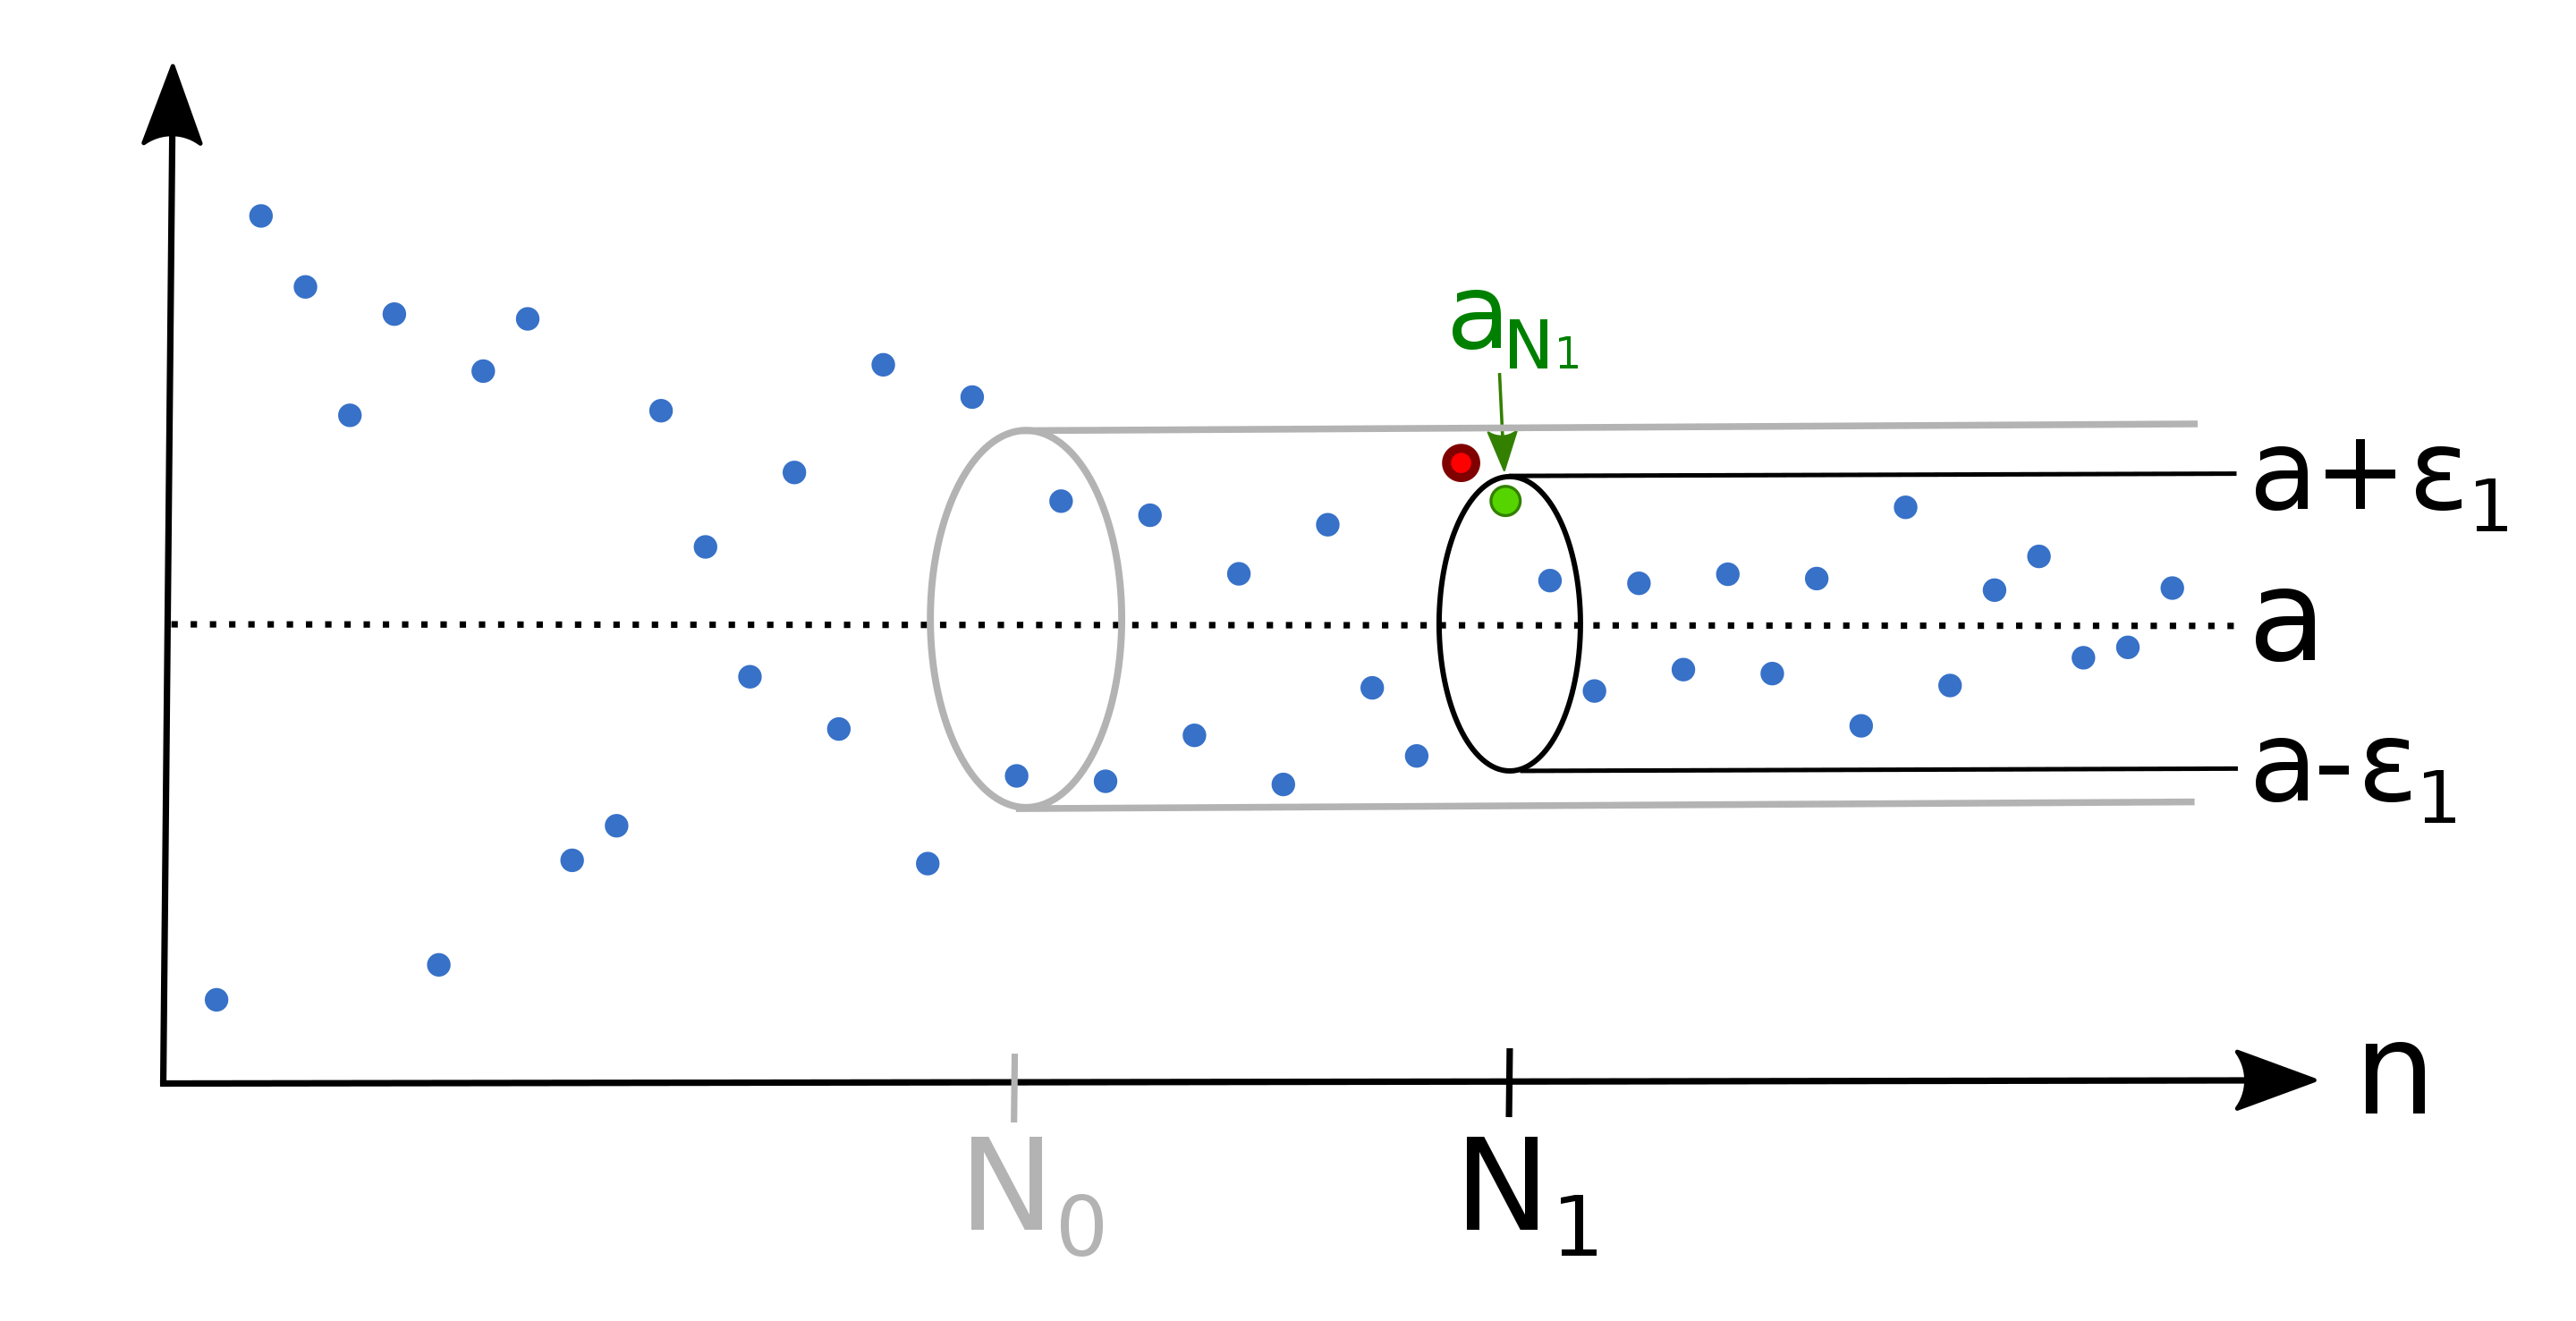
\includegraphics[width=\linewidth]{figures/limit.png}
    \caption{$a$ denotes the limit in this sequence, $N_0$ denotes $N(\epsilon_0)$ for some $\epsilon_0$, and $N_1 = N(\epsilon_1) < N_0$ for some $\epsilon_1 < \epsilon_0$.}
\end{figure}
\begin{exc}
    Prove that a sequence converges $\implies$ the sequence is Cauchy.
\end{exc}
\begin{defi}
    A metric space $(X,d)$ is complete if every Cauchy sequence converges.
\end{defi}

\begin{defi}[Open ball]
    An open $\e$-ball about $c$ is the set $B_{\e}(c) = \{x : d(x,c) < \e\}$.
\end{defi}
\begin{defi}[Accumulation point]
    Let $A \sse X$. Point $a$ is an accumulation point of $A$ if 
    \begin{align*}
        \forall \e > 0 \ \E x \in A: x \neq a \text{ and } x \in B_{\e}(a)
    \end{align*}
    In other words, every open $\e$-ball about $a$ contains a point from $A$ that is different from $a$.
\end{defi}
\begin{exm}
    Let $X = \R$. The set $A = [0, 1)$ has accumulation point 1, as every interval $B_{\e}(1) = (1 - \e, e + \e)$ contains a point in $[0,1)$.
\end{exm}
\begin{defi}[Open set]
    A set $A \sse X$ is called open if for every $x \in A$, $\E \e>0 : B_{\e}(x) \sse A$. In other words, for every point in $A$, a small enough open ball about that point is also in $A$.
\end{defi}
\begin{exm}
    Let $X = \R$. The set $A = (0, 1)$ open.
    \begin{proof}
    Formally, let $x \in (0,1)$. Let $\e = \min\{x, 1-x\}$. Then, $B_{\e}(x) \sse (0,1)$.
    \end{proof}
\end{exm}
\begin{exm}
    Any open ball is open.
    \begin{proof}
    Using the notation from the figure below, let $A = B_r(x)$ be an open ball in $(X,d)$. Choose $y \in A$. Let $\e = r - d(x,y)$. To show that $B_{\e}(y) \sse B_r(x)$, take any point $z \in B_{\e}(y)$. By construction, we have:
    \begin{align*}
        d(y, z) < \e = r - d(x,y) \implies d(y, z) + d(x, y) < r
    \end{align*}
    To show that $z \in B_r(x)$, we bound $d(x,z)$ by $r$.
    \begin{align*}
        d(x,z) \leq d(y, z) + d(x, y) < r
    \end{align*}
    \end{proof}
\end{exm}
\clearpage
\begin{figure}
    \centering
    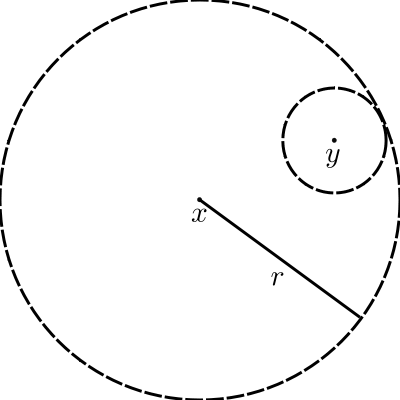
\includegraphics[width=0.5\linewidth]{figures/open_ball.png}
    \caption{An open $r$-ball about $x$. Dotted lines typically denote the unincluded boundary of the set.}
\end{figure}
\begin{defi}[Closed set]
    A set $A$ is closed if it contains all of its accumulation points.
\end{defi}
\begin{exm}
    As seen above, $[0,1)$ has (only) accumulation point 1. Thus the set $[0,1]$ is closed.
\end{exm}
\begin{thm}
    $A$ is open if and only if $A^c$ is closed.
\end{thm}
\begin{rem}
    In $\R$, the sets $\R$ and $\emptyset = \{\}$ are both open and closed.
\end{rem}
\begin{rem}
    A finite set $A = \{x_1, x_1, ..., x_n\}$ is closed. With distinct elements, no point is an accumulation point, thus all are contained.
\end{rem}
\begin{thm}
    The following hold in $(X,d)$.
    \begin{enumerate}
        \item An arbitrary number of unions of open sets is open.
        \item A finite number of intersections of open sets is open.
        \item A finite number of unions of closed sets is closed.
        \item An arbitrary number of intersections of closed sets is closed.
    \end{enumerate}
\end{thm}
\begin{exm}
    Let $A_n = (-\frac{1}{n}, \frac{1}{n})$. Each $A_n$ is open. However, $A = \bigcap_{n=1}^\infty A_n = \{0\}$ which is not open.
\end{exm}
\begin{exm}
    Let $A_n = \{\frac{1}{n}\}$. Each $A_n$ is closed. However, $A = \bigcup_{n=1}^\infty A_n = \{\frac{1}{n} : n = 1, 2, ..\}$, which has accumulation point 0, and is thus not closed. 
\end{exm}

\section{September 10, 2019}

\subsection{Real analysis review, cont'd}

\begin{defi}[Open cover]
    An open cover of set $A$ is a (possibly infinite) collection of open sets $\mathcal{S}$ such that $A \sse \bigcup_{O \in \mathcal{S}} O$. A subcover is a subset of $\mathcal{S}$ that is still a cover for $A$
\end{defi}
\begin{defi}[Compact set]
    The following are equivalent statements.
    \begin{enumerate}
        \item A set $A$ is compact.
        \item Every open cover of $A$ has a finite subcover.
        \item Every sequence $x_1, x_2,...$ with $x_n \in A$ has subsequence that converges to $x \in A$.
    \end{enumerate}
\end{defi}
\clearpage
\begin{figure}
    \centering
    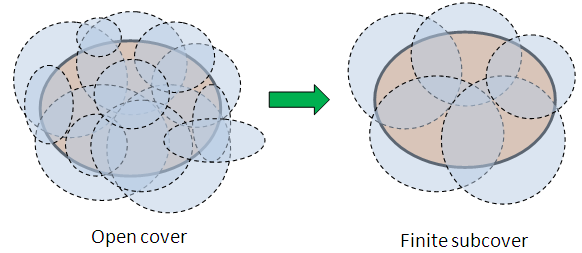
\includegraphics[width=0.8\linewidth]{figures/finite_subcover.png}
    \caption{The brown ellipse represents a set, and the blue ellipses represent an open cover. Note that compactness does not require the existence of an open cover, but for every given (even infinite) open cover, one can extract a finite subcover.}
\end{figure}
These definitions can be difficult to verify. In $\R^n$, there is a simpler characterization.
\begin{defi}[Boundedness]
    A set $A$ is bounded if there exists a point $c \in X$ with finite radius $r$ such that $A \sse B_r(c)$. In other words, $A$ is bounded if an open ball can contain it fully.
\end{defi}
\begin{thm}[Heine-Borel]
    $A \in \R^n$ is compact if and only if it is closed and bounded.
\end{thm}
\clearpage
\begin{figure}
    \centering
    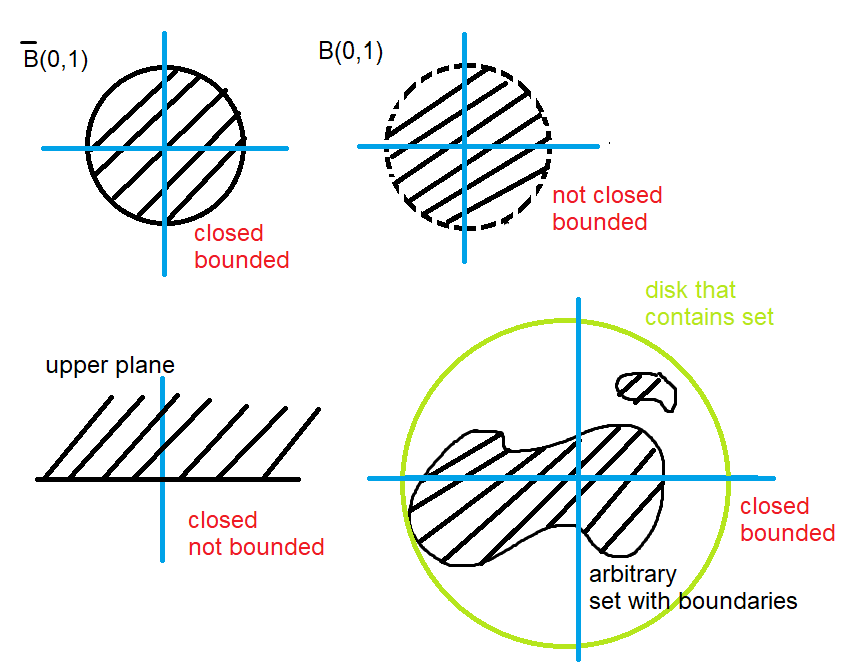
\includegraphics[width=\linewidth]{figures/compact.png}
    \caption{The shaded regions represent elements of the set, with solid and dotted boundaries denoting inclusion and exclusion, respectively. The top-left and bottom-right are compact sets in $\R^2$.}
\end{figure}
\begin{exm}
    In $\R$, a closed interval $[a, b]$ is compact.
\end{exm}
\begin{exm}
    In $\R^n$, the unit sphere $A = \{x : ||x||_2 = 1\}$ is compact (where $||x||_2 = \sqrt{\sum_{i=1}^n x_i^2}$).
\end{exm}
\begin{defi}[Continuity]
    Let $f: (X, d_X) \rightarrow (Y, d_Y)$. $f$ is continuous at $x_0$ if for every $\e > 0$, there is a $\delta(\e, x_0)$ such that $\forall x \in X$:
    \begin{align*}
        d(x, x_0) < \delta \implies d(f(x), f(x_0)) < \e
    \end{align*}
    $f$ is continuous if it is continuous at all $x_0 \in X$.
\end{defi}
The definition of continuity captures the notion that small changes in $x$ should result in small changes in $f(x)$. Specifically, the change in $f(x)$ should be made arbitrarily small by controlling the change in $x$. Note that $\delta$ depends on both $\e$ and $x_0$. 
\clearpage
\begin{figure}
    \centering
    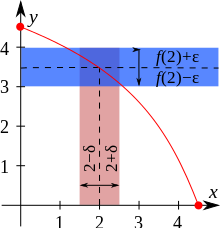
\includegraphics[width=0.5\linewidth]{figures/continuous.png}
    \caption{This function is continuous at $x = 2$.}
\end{figure}
\begin{defi}[Uniform continuity]
    Let $f: (X, d_X) \rightarrow (Y, d_Y)$. $f$ is uniformly continuous if for every $\e > 0$, there is a $\delta(\e)$ such that $\forall x_0, x_1 \in X$:
    \begin{align*}
        d(x_0, x_1) < \delta \implies d(f(x_0), f(x_1)) < \e
    \end{align*}
\end{defi}
Note that the dependence of $\delta$ on the point in $X$ is not gone.
\clearpage
\begin{figure}
    \centering
    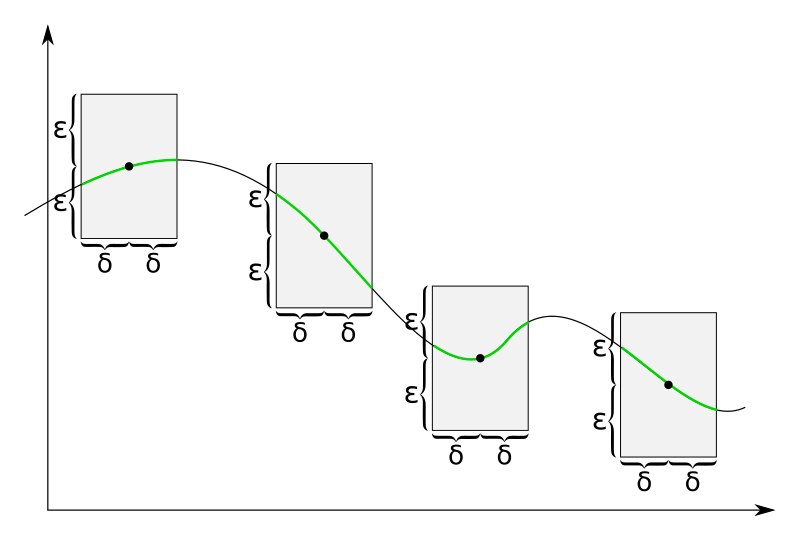
\includegraphics[width=0.494\linewidth]{figures/uniform.png}
    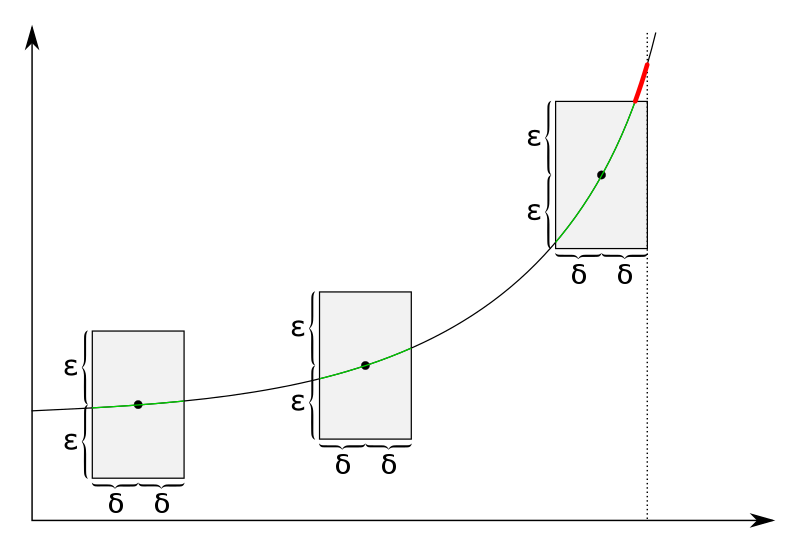
\includegraphics[width=0.494\linewidth]{figures/not_uniform.png}
    \caption{A pictorial characterization of continuity whether a ring of height $2\e$ and width $2\delta$ could slide along the entire function, without turning, for every $\e$. If $\delta$ must change as this happens, the the function is only continuous. In the right example, $\delta$ must get smaller as $x$ gets large in order for the ring to continue sliding. In the case that $\delta$ can stay constant, as in the left example, then the function is uniformly continuous.}
    \label{fig:cont}
\end{figure}

\section{September 17, 2019}

In response to questions from last time:
\begin{exc}
    Show that compactness implies closure in a metric space.
\end{exc}
\begin{exm}
    Show that compactness implies boundedness in a metric space.
    \begin{proof}
        Let $(X,d)$ be the metrix space, and $A$ be the compact set of interest. Chose any $x_0 \in X$, and write $\mathcal{S} = \{B_r(x_0) : r > 0\}$. Clearly, $A \subset \mathcal{S}$, and $\mathcal{S}$ is an open cover of $A$. Thus, there exists a finite subcover
        \begin{align*}
            F = \{B_{r_1}(x_0), ..., B_{r_p}(x_0)\}
        \end{align*}
        Take $r = \max_{i=1,...,p} r_i$, and $A \sse B_r(x_0)$.
    \end{proof}
\end{exm}
\begin{exc}
    Given an example of a metric space that is closed and bounded, but not compact. Hint: Use the discrete metric. That is,
    \begin{align*}
        d(x,y) = \begin{cases}
        0 \text{ if } x = y\\
        1 \text{ if } x \neq y
        \end{cases}
    \end{align*}
\end{exc}
\begin{exm}
    Prove that $f(x) = \frac{1}{x}$ on $x > 0$ is not uniformly continuous.
    \begin{proof}
        Let $\e = 1$. For any $\delta$, we must choose $x_0$ and $x_1$ such that $|x_0 - x_1| < \delta$ does imply that $|f(x_0) - f(x_1)| < 1$.
        \begin{align*}
            |f(x_0) - f(x_1)| = \frac{\delta}{x_0 x_1}
        \end{align*}
        Letting $x_1 = x_0 + \frac{\delta}{2}$.
        \begin{align*}
            |f(x_0) - f(x_1)| = \frac{\delta}{x_0 (x_0 + \frac{\delta}{2})}
        \end{align*}
        Choosing $x_0$ small enough can make this quantity larger than $\e = 1$.
    \end{proof}
\end{exm}

Continuing with the review, there are many useful properties that result from a continuous function on a compact set.
\begin{thm}
    Let $f: (X,d_X) \rightarrow (\R, d_Y)$ be continuous over compact set $X$. Then:
    \begin{enumerate}
        \item $f$ is uniformly continuous.
        \item $f(X) = \{f(x) : x \in X\}$ is compact. 
        \item $f$ achieves $\max_{x \in X} \{f(x)\}$ and $\min_{x \in X} \{f(x)\}$, as in there exists $x^*_{\text{max}}, x^*_{\text{min}} \in X$ such that
        \begin{align*}
            f(x^*_{\text{min}}) \leq f(x) \leq f(x^*_{\text{max}})
        \end{align*}
        for all $x$.
        \item Let $\lim_{n \rightarrow \infty} x_n = x$, where $x_n, x \in X$. Then
        \begin{align*}
            \lim_{n \rightarrow \infty} f(x_n) = f\left(\lim_{n \rightarrow \infty} x_n\right) = f(x)
        \end{align*}
    \end{enumerate}
\end{thm}
\begin{exm}
    Let $f: (X,d_X) \rightarrow (Y, d_Y)$ and $g: (Y,d_Y) \rightarrow (Z, d_Z)$ both be continuous functions. Show that the composition $f \circ g$ is continuous.
    \begin{proof}
        Given any $x_0 \in X$ and any $\e > 0$, let $y_0 = f(x_0)$. Choose $\delta_g(\e, y_0)$ such that:
        \begin{align*}
            d_Y(y_0,y) < \delta_g \implies d_Z(g(y_0), g(y)) < \e
        \end{align*}
        Then choose $\delta_f(\delta_g, x_0)$ such that:
        \begin{align*}
            d_X(x_0,x) < \delta_f \implies d_Y(f(x_0),f(x)) < \delta_g
        \end{align*}
        Thus
        \begin{align*}
             d_X(x_0,x) < \delta_f \implies d_Y(f(x_0),f(x)) < \delta_g \implies d_Z(g(f(x_0)), g(f(x))) < \e
        \end{align*}
    \end{proof}
\end{exm}
\begin{exc}
    Give a function that is bounded, i.e. there is some $B \geq 0$ such that $|f(x)| \leq B$ for all $x \in X$, and continuous, but not uniformly continuous.
\end{exc}
\begin{defi}[Lipshitz continuity]
    A function $f: (X,d_X) \rightarrow (Y, d_Y)$ is called Lipshitz continuous with Lipshitz constant $L$ for all $x_0, x_1 \in X$:
    \begin{align*}
        d_Y(f(x_0), f(x_1)) \leq L \cdot d_X(x_0, x_1)
    \end{align*}
\end{defi}
This means that the changes in $f(x)$ are sublinear in the changes in $x$. The constant $L$ ``quantifies" the continuity of $f$. 
\begin{obs}
    Lipshitz continuity implies uniform continuity.
    \begin{proof}
        Given any $e > 0$, let $\delta = \frac{\e}{L}$.
        \begin{align*}
            d_Y(f(x_0), f(x_1)) \leq L \cdot d_X(x_0, x_1) \leq L \cdot \frac{\e}{L} = \e
        \end{align*}
    \end{proof}
\end{obs}

Pointers for Homework 1:
\begin{enumerate}
        \item Similarity implies sameness of rank, spectrum/charactaristic polynomial and determinant. None of the reverse implications hold.
        \item Same eigenvectors does not imply similarity. What does it imply (assuming there are $n$ of them that are linearly independent)?
        \item What can you say about a matrix with distinct eigenvalues?
        \item What can you say about the eigenvalues of diagonal/triangular matrix?
        \item A matrix is invertible - what can you say about its eigenvalues?
\end{enumerate}

\section{September 24, 2019}

{\it Homework 1 solutions.}

\section{October 1, 2019}

{\it Homework 2 solutions.}

\section{October 8, 2019}

{\it Copies of Homework 3 solutions distributed.}\\

When I say "application", I mean that these topics are not tested in the course, but topics mostly from mathematical data science that are interesting and make use of material from the course.

\subsection*{Application: Projection Matrices} 

$A^2 = A \in M_n(\R)$. What can you say about this matrix? Given the additional information that $A = A^T$, what else can be said?

The matrix has annihilating polynomial $p(t) = t(t-1)$, therefore any eigenvalues $\lambda \in \{0,1\}$. $q_A$ divides this polynomial, so $q_A$ is the product of distinct linear factors, implying that $A$ is diagonalizable. In fact $Ax = SDS^{-1}x$ is a projection of $x$ onto the subspace spanned by the eigenvectors of $A$ associated with eigenvalue 1. This happens in three steps.
\begin{enumerate}
    \item $y_1 = S^{-1}x$ gives the coordinates of $x$ in the basis described by the columns of $A$.
    \item $y_2 = Dy_1$ scales the components by 0 or 1, eliminating certain dimensions and keeping other.
    \item $y_3 = Sy_2$ brings us back into the original basis.
\end{enumerate}
If $A = A^T$, then it is real orthogonally diagonalizable, with the eigenvectors forming an orthonormal basis. This idea is depicted in Figure \ref{fig:proj}. The transformation $A$ is called a projection matrix. The next topic will make use of ideas from Chapters 0 through 4.

\begin{figure}[ht!]
    \centering
    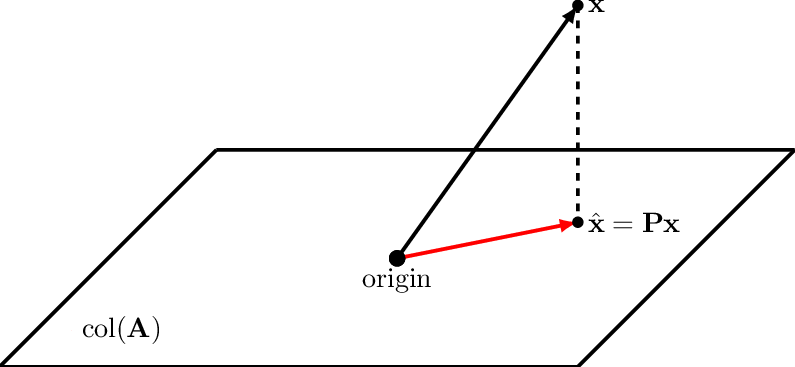
\includegraphics[width=0.6\linewidth]{figures/projection.png}
    \caption{Here ${\bf x} \in \R^3$ is the vector of interest and ${\bf P} \in M_3(\R)$ is the projection matrix. If we ${\bf P} = SDS^{-1}$ let ${\bf A}$ be the $M_{3,2}(\R)$ matrix that column binds the eigenvectors of ${\bf P}$ associated to eigenvalue 1, then the subspace column space of ${\bf A}$.}
    \label{fig:proj}
\end{figure}

\subsection*{Application: numerical optimization}

Let $f: \R^d \rightarrow \R$ be a twice-differentiable function, with
\begin{align*}
    \nabla f(x) &=: g(x) \in \R^d\\
    \nabla^2 f(x) &=: H(x) \in M_d(\R)
\end{align*}
\begin{defi}[Local minimum]
    $x^*$ is a local minimum of $f$ if there exists an $\e > 0$ such that for all $x \in B_{\e}(x)$, $f(x^*) \leq f(x)$.
\end{defi}

Our goal is to find such a local minimum, and we write this problem as
\begin{align*}
    \min_{x \in \R^d} f(x)
\end{align*}

There are many ways to go about this, but one such was is to iteratively propose candidate solutions $x_1, x_2, ...$ that get ``closer" to a local minimum $x^*$. A subset of these methods is line-search methods, where at iterate $x_t$, we choose a search direction $p \in \R^d$ and step size $\alpha \in [0, 1)$, and let $x_{t+1} = x_t + \alpha p$. For example, in gradient descent, we let $p = - g(x_t)$, as in Figure \ref{fig:grad}.
\begin{figure}[ht!]
    \centering
    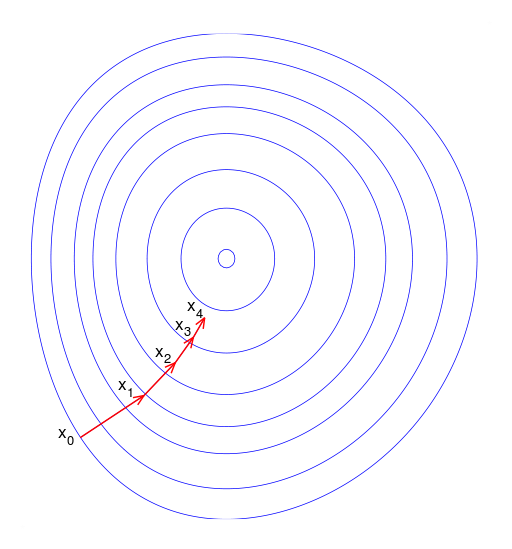
\includegraphics[width=0.5\linewidth]{figures/grad.png}
    \caption{The center of the contour plot is the local minimum.}
    \label{fig:grad}
\end{figure}

Some basic optimality conditions:
\begin{align*}
    \text{$x^*$ is a local minimum.} &\implies g(x^*) = 0 \text{ and  $H(x)$ is P.S.D.}\\
    g(x^*) = 0\text{ and  $H(x)$ is P.D.} &\implies \text{$x^*$ is a local minimum.}
\end{align*}
While we will not prove them, we will attempt to understand them via the Hessian matrix $H(x^*)$. Taylor expand $f(x_0 + \alpha p)$ about $x_0$.
\begin{align*}
    f(x_0 + \alpha p) = f(x_0) + \alpha g(x_0)^T p + \frac{1}{2} \alpha^2 p^T H(x_0) p + o(\alpha^2)
\end{align*}
Assume that we are at a stationary point $x_0$, i.e. $g(x_0) = 0$. Note that $H = H^T$ for any $x$, thus $H$ is real orthogonally diagonalizable. Let $u_1, ..., u_d$ be the eigenvectors of $H(x_0)$. Start by considering $p = u_k$.
\begin{align*}
    f(x_0 + \alpha u_k) &= f(x_0) + \alpha g(x_0)^T u_k + \frac{1}{2} \alpha^2 u_k^T H(x_0) u_k + o(\alpha^2)\\
    \implies f(x_0 + \alpha u_k) - f(x_0) &= \frac{1}{2} \alpha^2 \lambda_k + o(\alpha^2)
\end{align*}
where $\lambda_k$ is the eigenvalue associated to $u_k$. It's clear that for small $\alpha$, if $\lambda_k$ is positive, then the function will increase, where as for negative $\lambda_k$, the function will decrease. For $\lambda_k = 0$, the higher-order terms determine the sign of the change in function value.

Now consider arbitrary search direction $p$. Because $H = H^T$, the eigenvectors of $H$ for an othonormal basis for $\R^d$, and we can write
\begin{align*}
    p &= UU^Tp\\
    &= (u_1^T p) u_1 + ... + (u_d^T p) u_d\\
    &= \sum_{k=1}^d (u_k^T p) u_k
\end{align*}
Then, the the Taylor expansion gives us
\begin{align*}
    f(x_0 + \alpha u_k) - f(x_0) &= \frac{1}{2} \alpha^2 \sum_{k=1}^d (u_k^T p)^2 \lambda_k + o(\alpha^2)
\end{align*}
Thus, the change in the function is a weighted sum of the eigenvalues of $H(x_0)$, weighted by how parallel the search direction is with the associated eigenvector. If all $\lambda_k > 0$ (i.e. $H(x_0)$ is P.D.) then there is nothing to worry about, and every direction will increase the function value for small enough $\alpha$. This is just another way of saying that we are at a local minimum. However, any negative eigenvalue reveals a descent direction, and if an eigenvalue is 0, then the higher-order term $o(\alpha^2)$ could still decrease the function (which is why $H(x_0)$ P.S.D. is not sufficient). 

Finally, we answer the following question: what is the interpretation of $D$? Assume that $f(x)$ is a quadratic form, in that $f(x) = b + g^Tx + \frac{1}{2}x^T H x$ for $b \in \R$,  $x, g \in \R^d$, and $H \in M_d(\R)$ symmetric (why can we make $H$ symmetric without loss of generality?). Let $f_U(x) = f(U^T x)$.
\begin{align*}
    \nabla^2 f_U(x) &= U^T \nabla^2 f(U^T x) U\\
    &= U^T H U\\
    &= D
\end{align*}
For a quadratic function, letting $H = UDU^T$, $D$ is the Hessian of the function evaluated in a rotated basis.

Another important point is that eigenvalues of large magnitude have eigenvectors which are direction of steep increase or decrease, as suggested by the Taylor expansion. We will come back to this point when we discuss condition number, specifically how different ratios of eigenvalues affects the success of optimization algorithms. 

As a final message: in applications related to mathematical data science, when we see (say square) matrices, if you gain anything from this class it will be the willingness and ability to answer the following two questions.
\begin{enumerate}
    \item If the matrix is symmetric (Hermitian, normal), what is the  interpretation of its eigenvalues and eigenvectors? What is the interpretation of the diagonal matrix $D$?
    \item Is the matrix full-rank, low-rank, or approximately low-rank? What are the implications of each case? What is its condition number, and what are its implications?
\end{enumerate}

By approximately low-rank, we mean eigenvalues (or more generally, singular values) small in magnitude. The second question we will be able to attack more after Chapter 7 and 5, but the first we can start understanding now. 

\section{October 15, 2019}

\subsection*{Announcements}

Exam 1 just passed, and I unfortunately do not have the answer to the following questions.
\begin{itemize}
    \item I got grade $x$ on Exam 1, will I still be able to get grade $y$ in the class?
    \item Are Exams 2 and 3 easier than Exam 1?
\end{itemize}
The first question I will direct to Dr. Fishkind, while for the second, the best answer I can offer is that I looked at the exam scores from last years, and students performed statistically significantly better on Exam 2 and 3 than on Exam 1. However, operationally, the average was 4 points higher on Exam 2 and 8 points higher on Exam 3, so take that as you will. It is likely that students' expectations are better calibrated for future exams, rather than them being easier.

\subsection*{Some chapter 4 results}

\begin{thm}
    Let $A \in M_n$ be normal. Let $F(A) = \{\frac{x^* A x}{x^* x} : x \in \C^n \backslash \{0\}\}$. Then $F(A) = \mathcal{H}(A)$, where $\mathcal{H}(\cdot)$ denotes the convex hull.
\end{thm}

\begin{thm}[Rayleigh-Ritz]
    Let $A \in M_n$ be Hermitian, with (orthonormal) eigenvectors $u_1, ..., u_n$, associated with $\lambda_1 \leq ... \leq \lambda_n$. For $k = 1, ..., n$, we have:
    \begin{align*}
        \min_{\substack{x \neq 0 \\ x \perp u_1 ,..., u_{k-1}}} \frac{x^* A x}{x^* x} &= \lambda_k\\
        \max_{\substack{x \neq 0 \\ x \perp u_{k+1} ,..., u_n}} \frac{x^* A x}{x^* x} &= \lambda_k
    \end{align*}
\end{thm}
\begin{proof}
    We'll prove the maximum case. Represent any such $x$ as
    \begin{align*}
        x = \delta_{1} u_{1} + ... + \delta_k u_k = \sum_{i=1}^k \delta_i u_i
    \end{align*}
    with not all $\delta_i$ equal to 0. Let $A = UDU^*$ be the unitary diagonalization.
    \begin{align*}
        \max_{\substack{x \neq 0 \\ x \perp u_{k+1} ,..., x_n}} \frac{x^* A x}{x^* x} &= \max_{\delta_1, ..., \delta_k} \frac{(\sum_{i=1}^k \delta_i u_i)^* U D U^* \sum_{i=1}^k \delta_i u_i}{(\sum_{i=1}^k \delta_i)^* (\sum_{i=1}^k \delta_i)}\\
        &= \max_{\delta_1, ..., \delta_k} \frac{(\sum_{i=1}^k \overline{\delta_i} u_i^* U) D (\sum_{i=1}^k \delta_i U^* u_i)}{\sum_{i=1}^k \overline{\delta_i} \delta_i}\\
        &= \max_{\delta_1, ..., \delta_k} \frac{\begin{bmatrix}
            \overline{\delta_1} & \ldots & \overline{\delta_k} & 0 & \ldots & 0
        \end{bmatrix}
        \begin{bmatrix}
            \lambda_1 & & & & &\\
            & \ddots & & & &\\
            & & \lambda_k & & &\\
            & & & \lambda_{k+1} & &\\
            & & & & \ddots &\\
            & & & & & \lambda_n
        \end{bmatrix}
        \begin{bmatrix}
            \delta_1 \\ \vdots \\ \delta_k \\ 0 \\ \vdots \\ 0
        \end{bmatrix}}{\sum_{j=1}^k |\delta_j|^2}\\
        &= \max_{\delta_1, ..., \delta_k} \sum_{i=1}^k \frac{|\delta_i|^2}{\sum_{j=1}^k |\delta_j|^2} \lambda_i\\
        &= \lambda_k
    \end{align*}
\end{proof}

\begin{thm}[Courant-Fischer]
    Let $A \in M_n$ be Hermitian. Then
    \begin{align*}
        \max_{y_1 ,..., y_{k-1}} \phi_{\min}(y_1, ..., y_{k-1}) = \max_{y_1 ,..., y_{k-1}} \min_{\substack{x \neq 0 \\ x \perp y_1 ,..., y_{k-1}}} \frac{x^* A x}{x^* x} &= \lambda_k\\
        \min_{y_{k+1} ,..., y_n} \phi_{\max}(y_{k+1}, ..., y_n) = \min_{y_{k+1} ,..., y_n} \max_{\substack{x \neq 0 \\ x \perp y_{k+1} ,..., y_n}} \frac{x^* A x}{x^* x} &= \lambda_k
    \end{align*}
\end{thm}
\begin{proof}
    We show the first equality. Noting that $y_1, ..., y_{k-1}$ are not necessarily linearly independent, and letting $u_1, ..., u_k, ..., u_n$ be the eigenvectors of $\lambda_1 \leq ... \leq \lambda_k \leq ... \leq \lambda_n$, we have
    \begin{align*}
        \text{dim} \ \text{span}\{y_1, ..., y_{k-1}\} &\leq k - 1\\
        \implies \text{dim} \ \text{span}\{y_1, ..., y_{k-1}\}^{\perp} &\geq n - (k - 1) = n - k + 1\\
        \text{dim} \ \text{span}\{u_1, ..., u_k\} &= k\\
    \end{align*}
    Thus
    \begin{align*}
        \text{dim} \ \text{span}\{y_1, ..., y_{k-1}\}^{\perp} + \text{dim} \ \text{span}\{u_1, ..., u_k\} \geq n + 1
    \end{align*}
    So the intersection $\text{span}\{y_1, ..., y_{k-1}\}^{\perp} \cap \text{span}\{u_1, ..., u_k\}$ must have some nonzero vectors. Let $w \neq 0$ be one such vector. We have
    \begin{align*}
        w \perp u_{k+1}, ..., u_n,
    \end{align*}
    and so by Rayleigh-Ritz,
    \begin{align*}
        \frac{w^* A w}{w^* w} \leq \lambda_k \implies \min_{\substack{w \neq 0 \\ w \perp y_1 ,..., y_{k-1} \\ w \perp u_{k+1}, ..., u_n}} \frac{w^* A w}{w^* w} \leq \lambda_k
    \end{align*}
    This also means that
    \begin{align*}
        \phi_{\min}(y_1, ..., y_{k-1}) = \min_{\substack{x \neq 0 \\ x \perp y_1 ,..., y_{k-1}}} \frac{x^* A x}{x^* x} \leq \min_{\substack{w \neq 0 \\ w \perp y_1 ,..., y_{k-1} \\ w \perp u_{k+1}, ..., u_n}} \frac{w^* A w}{w^* w} \leq \lambda_k
    \end{align*}
    and thus we have found an upper bound for $\phi_{\min}(y_1, ..., y_{k-1})$. Setting $y_1 = u_1, ..., y_{k-1} = u_{k-1}$, we achieve this upper bound, and thus
    \begin{align*}
        \max_{y_1 ,..., y_{k-1}} \phi_{\min}(y_1, ..., y_{k-1}) = \max_{y_1 ,..., y_{k-1}} \min_{\substack{x \neq 0 \\ x \perp y_1 ,..., y_{k-1}}} \frac{x^* A x}{x^* x} &= \lambda_k\\
    \end{align*}
    as desired. As for the second equality (which is entirely analogous), we have
    \begin{align*}
        \text{dim} \ \text{span}\{y_{k+1}, ..., y_n\} &\leq n - k\\
        \implies \text{dim} \ \text{span}\{y_{k+1}, ..., y_n\}^{\perp} &\geq n - (n - k) = k\\
        \text{dim} \ \text{span}\{u_k, ..., u_n\} &= n - k + 1\\
    \end{align*}
    Thus
    \begin{align*}
        \text{dim} \ \text{span}\{y_{k+1}, ..., y_n\}^{\perp} + \text{dim} \ \text{span}\{u_k, ..., u_n\} \geq n + 1
    \end{align*}
    So the intersection $\text{span}\{y_{k+1}, ..., y_n\}^{\perp} \cap \text{span}\{u_k, ..., u_n\}$ must have some nonzero vectors. Let $w \neq 0$ be one such vector. We have
    \begin{align*}
        w \perp u_1, ..., u_{k-1},
    \end{align*}
    and so by Rayleigh-Ritz,
    \begin{align*}
        \frac{w^* A w}{w^* w} \geq \lambda_k \implies \max_{\substack{w \neq 0 \\ w \perp y_{k+1} ,..., y_n \\ w \perp u_1, ..., u_{k-1}}} \frac{w^* A w}{w^* w} \geq \lambda_k
    \end{align*}
    This also means that
    \begin{align*}
        \phi_{\max}(y_{k+1}, ..., y_n) = \max_{\substack{x \neq 0 \\ x \perp y_{k+1}, ..., y_n}} \frac{x^* A x}{x^* x} \geq \max_{\substack{w \neq 0 \\ w \perp y_{k+1}, ..., y_n \\ w \perp u_1, ..., u_{k-1}}} \frac{w^* A w}{w^* w} \geq \lambda_k
    \end{align*}
    and thus we have found a lower bound for $\phi_{\max}(y_{k+1}, ..., y_n)$. Setting $y_{k+1} = u_{k+1}, ..., y_n = u_n$, we achieve this lower bound, and thus
    \begin{align*}
        \min_{y_{k+1},..., y_n} \phi_{\max}(y_{k+1}, ..., y_n) = \min_{y_{k+1},..., y_n} \max_{\substack{x \neq 0 \\ x \perp y_{k+1}, ..., y_n}} \frac{x^* A x}{x^* x} &= \lambda_k\\
    \end{align*}
    as desired.
\end{proof}

\begin{thm}[Weyl]
    Let $A, B \in M_n$ be Hermitian. Then, for all $k = 1, ..., n$
    \begin{align*}
        \lambda_k(A) + \lambda_1(B) \leq \lambda_k(A + B) \leq \lambda_k(A) + \lambda_n(B)
    \end{align*}
    where $\lambda_i(A)$ is the $i$-th smallest eigenvalue of $A$.
\end{thm}

\begin{coro}
    Let $A, B \in M_n$ be P.S.D.. Then for all $k = 1, ..., n$,
    \begin{align*}
        \lambda_k(A) \leq \lambda_k(A + B)
    \end{align*}
\end{coro}

\begin{rem}
    For $a \in \{-1, 1\}, y \in \C^n \backslash \{0\}$, $ayy^*$ is a rank 1 Hermitian matrix. Any rank 1 Hermitian matrix can be written as such.
\end{rem}
\begin{thm}[Interlacing I]
    For $A$ Hermitian, $a \in \{-1, 1\}, y \in \C^n \backslash \{0\}$, then for all $k$,
    \begin{align*}
        \lambda_k(A + ayy^*) \leq \lambda_{k+1}(A) 
    \end{align*}
\end{thm}

\begin{thm}[Interlacing II]
    Let $A \in M_n$ be Hermitian, $B \in M_r$ be a principal submatrix of $A$. Then for all $k$ such that $1 \leq k \leq r$,
    \begin{align*}
        \lambda_k(A) \leq \lambda_k(B) \leq \lambda_{k+n-r}(A)
    \end{align*}
\end{thm}

\begin{coro}
    If $A \in M_n$ is Hermitian, and $a_{ii}$ is on the diagonal, then
    \begin{align*}
        \lambda_1(A) \leq a_{ii} \leq \lambda_n
    \end{align*}
\end{coro}

\subsection*{Application: multivariate statistics}

In the interest of time, and the fact that there are many resources on this subject, we may not go over the statistics example fully in class. However, here is the setup and the questions, and you can answer them on your own and discuss in office hours!

Let $x: \Omega \rightarrow \R^d$ and $x \in \R^d$ both represent a $d$-dimensional random variable and its realization. The distinction should be clear from context. Let $\EV[x] = \mu$ be the mean and $\text{Cov}[x] = \EV[(x - \mu)(x - \mu)^T] = \Sigma$ be the (Hermitian) covariance matrix.
\begin{enumerate}
    \item Prove that $\Sigma$ is P.S.D.. Why is it not P.D. in general?
    \item Interpret the eigenvectors, eigenvalues, and diagonal matrix $D$.
    \item Let $x \sim \mathcal{N}(\mu, \Sigma)$. Prove that $\Sigma$ is in fact P.D.. Plot the probability density function for $d = 2$ and use the optimization example to interpret the shape.
    \begin{itemize}
        \item Why does a large eigenvalue $\lambda_k$ correspond to a large spread in $u_k$ (meaning large value of $\text{Var}(||\text{proj}_{u_k}(x)||)$)?
        \item For what values of the spectrum of $\Sigma$ are the level sets spherical versus oblong?
        \item When are the major axes of the level sets aligned with the coordinate axes?
    \end{itemize}
    \item If $x \sim \mathcal{N}(\mu, \Sigma)$ and $\Sigma = UDU^T$, what is the distribution of $z = U^T x$? Interpret $z$.
    \item Let $X \in M_{n, d}(\R)$ be a data matrix, where each row $x^T_i$ is an independent observation of $x$. Assume for simplicity that $\EV[x] = 0$. Finally, let $\frac{1}{n} X^T X = \hat{U} \hat{D}\hat{U}^T$ be an estimate of the unitary diagonalization of $\Sigma$. Consider two dimension reduction routines.
    \begin{itemize}
        \item Represent the data as $Z = X\hat{U}$, i.e. the principal components of $X$. Then, drop $d - r$ columns by some method.
        \item Drop columns from the {\it original} data matrix $X$ to $X_r$, then orthogonalize the reduced covariance matrix $\frac{1}{n} X_r^T X_r = \hat{U}_r \hat{D}_r\hat{U}^T_r$. Represent the reduced data as $Z_r = X_r \hat{U}_r$.
    \end{itemize}
    What is the conceptual difference between these two methods, that is, orthogonalizing and then dropping columns (of which PCA is an example) or vice versa? (Hint: use Interlacing II.)
\end{enumerate}

\section{October 22, 2019}

\subsection*{Exercises in section}

\begin{enumerate}
    \item What can be said about the diagonal elements of a skew Hermitian matrix?
    \item Let $A \in M_n$ be Hermitian. Prove that $A = A_+ + A_-$, where
    \begin{itemize}
        \item $A_+$ is P.S.D. and $A_-$ is N.S.D.,
        \item rank($A$) = rank($A_+$) + rank($A_-$), and 
        \item $A_+ A_- = A_+ A_- = 0$.
    \end{itemize}
    \item Prove that
    \begin{itemize}
        \item if $A$ is Hermitian, then $A^2$ is P.S.D.
        \item if $A$ is skew Hermitian, then $A^2$ is N.S.D.
    \end{itemize}
    \item Let $\mathcal{H}_n$ be the Hermitian matrices in $M_n$. $A \succeq B$ for $A, B \in \mathcal{H}_n$ if $A - B$ is P.S.D.. Prove that this is a partial ordering on $\mathcal{H}_n$, in that
    \begin{itemize}
        \item $A \succeq A$,
        \item $A \succeq B$ and $B \preceq A \iff A = B$, and
        \item $A \succeq B$ and $B \succeq C \implies A \succeq C$.
    \end{itemize}
    Why is $\mathcal{H}_n$ not totally ordered?
    \item Let $A \in M_n$ be Hermitian with exactly one positive and one negative eigenvalue. Explain why $\lambda_2(A) \geq 0$ and $\lambda_{n-1}(A) \leq 0$ with equality if and only if $n > 2$.
    \item Prove that the inner minimization and maximization of Courant-Fishcher always exists. That is, for any $A \in M_n$, $y_{1}, ..., y_{m}$ with $m < n$,
    \begin{align*}
        \inf_{x \neq 0, \ x \perp y_{1}, ..., y_{m}} \frac{x^* A x}{x^*x} \ \text{ and } \ \sup_{x \neq 0, \ x \perp y_{1}, ..., y_{m}} \frac{x^* A x}{x^*x}
    \end{align*}
    are achieved and can be replaced by minimum and maximum, respectively. You can take for granted that the matrix $z^* A z$ is continuous in $z$, with respect to the metric $d(z_0, z_1) = ||z_0 - z_1||$ where $||\cdot||$ is the Euclidean norm. We will be able to show this rigorously in Chapter 5.)
\end{enumerate}

We'll give a proof for the infimum in part (f), as to start getting used to the real analysis style proofs. 
\begin{proof}
First we note that
\begin{align*}
    \frac{x^* A x}{x^*x} = \frac{x^* A x}{||x||^2} = \left(\frac{x}{||x||}\right)^* A \left(\frac{x}{||x||}\right)
\end{align*}
$\frac{x}{||x||}$ is a unit vector, so we can just search values of $z^* A z$ over unit vectors $z$. Similarly, $x \perp y_{1}, ..., y_{m}$ if and only if $\frac{x}{||x||} \perp y_{1}, ..., y_{m}$, as scaling the length does not affect orthogonality (for non-zero vectors). Thus,
\begin{align*}
    \inf_{x \neq 0, \ x \perp y_{1}, ..., y_{m}} \frac{x^* A x}{x^*x} = \inf_{||z||_2 = 1, \ z \perp y_{1}, ..., y_{m}} z^* A z
\end{align*}
Using the hint that $z^* A z$ is continuous, we can show the existence of the infimum if the search space is compact. It is clear that the unit sphere $\{z : ||z|| = 1\}$ is compact. On the other hand, the set $\{z: z \perp y_{1}, ..., y_{m}\}$ is a subspace of dimension $l \leq m$. The search space is the intersection of these two sets. See Figure \ref{fig:sphere} for an example.
\begin{figure}[ht!]
    \centering
    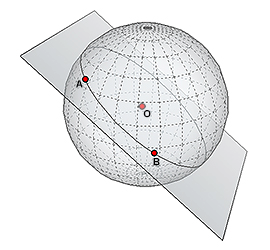
\includegraphics[width=0.7\linewidth]{figures/sphere-and-plane.png}
    \caption{Let $O$ be the origin, and $y$ 
    (not shown) be a vector normal to the plane. Then, $A$ and $B$ are two points in the intersection. They are both of unit length, and both orthogonal to $y$.}
    \label{fig:sphere}
\end{figure}
The subspace is represented by a hyperplane that crosses the origin. The intersection of an $l$-dimensional subspace and an $n$-dimensional unit sphere is an $l$-dimensional unit sphere. This is still a compact set, completing the proof that the inf (and sup) exist, which can now be replaced by min (and max).
\end{proof}

Pointers for Homework 4:
\begin{enumerate}
        \item What relationship can you advance about the set of Hermitian matrices and the set of skew Hermitian matrices?
        \item If $x \in \R^n$ majorizes $y \in \R^n$, what can you say about $x_1$ and $y_1$ (by definition) and about $x_n$ and $y_n$ (by inspection)?
        \item What can you say about any commuting matrices? If they are normal?
        \item Remember that in constructing principle submatrices, the undeleted rows/columns need not be contiguous. That is, for $n = 10$, I can delete rows/columns 1 - 3 and 5 - 7. This generates a submatrix of rows/columns 4, 8, 9, and 10.
        \item The leading principle submatrices $A_1, A_2, ..., A_n$ of $A$ are by definition principle submatrices of $A$. What else is true about them?
        \item For Problem 7, you should have a clear and specific analogue for Rayleigh-Ritz, Courant-Fischer, Interlacing I and II (and consequences), Weyl's theorem, and the majorization results.
\end{enumerate}

\section{October 29, 2019}

The theme of this section is understanding the singular value decomposition (SVD) of common data matrices. In statistics and machine learning, the data matrix (or design matrix) $X \in M_{n, d}(\R)$ has {\bf rows} $x^{(1)}, ..., x^{(n)} \in \R^d$ where each $x^{(i)}$ is an observation of some random vector
\begin{align*}
    x: \Omega \rightarrow \R^d
\end{align*}
with mean
\begin{align*}
    \mu = \EV[x] \in \R^d
\end{align*}
and covariance matrix
\begin{align*}
    \Sigma = \Cov(x) = \EV[(x - \mu)(x - \mu)^T] = \EV[xx^T] - \EV[x]\EV[x^T]
\end{align*}
This is analogous to the variance formula for univariate $x$, i.e. $\Var(x) = \EV[x^2] - \EV[x]^2$. We will just be thinking about the real version of these objects, but for complex numbers the analysis is the same, replacing transpose with conjugate transpose. Another data matrix we will visit is a grayscale image $P \in M_{m,n}(\R)$. 

We first will compare the SVD and eigendecomposition of an arbitrary Hermitian matrix $A$. If $A = UDU^*$ and $A^* = UD^*U = UDU^*$, then
\begin{align*}
    AA^* = U D U^* U D ^* = U D^2 U^*
\end{align*}
meaning that $A$ and $AA^*$ share the same eigenvectors, with $AA^*$ having the same eigenvalues, but squared. The ``$U$" matrix of the eigendecomposition of $AA^*$ is the same as the ``$U$" of the SVD of $A$, by definition.
\begin{align*}
    A = U \Sigma V^*
\end{align*}
What about $\Sigma$? Also by definition, we have that
\begin{align*}
    \Sigma = (D^2)^{\frac{1}{2}} = |D| = D \cdot \text{sgn}(D)
\end{align*}
where the $|\cdot|$ denotes element-wise absolute value, and $\text{sgn}(\cdot)$ is the element-wise sign function. 
\begin{align*}
    \text{sgn}(t) = \begin{cases}
    +1 &\text{ if } t > 0\\
    0 &\text{ if } t = 0\\
    -1 &\text{ if } t < 0
    \end{cases}
\end{align*}
Thus we can write
\begin{align*}
    UDU^* = A = U \Sigma V^* = U D \cdot \text{sgn}(D) V^*
\end{align*}
If $A$ is invertible, then $D$ is invertible, and we can conclude by cancelling out $UD$ that
\begin{align*}
    U^* = \text{sgn}(D) V^*
\end{align*}
Thus, the rows of $V^*$ are just equal to the rows of $U^*$, down to a sign. Where $A$ has a positive eigenvalue $\lambda_i$, the rows $u_i^*$ and $v_i^*$ will agree. Where $A$ has a negative eigenvalue $\lambda_i$, then $u_i^* = -v_i^*$. If $D$ is not invertible, then there will be zeros in $\text{sgn}(D)$, but if that is the case, then it doesn't really matter what is in those rows of $U^*$ and $V^*$ (as long as they are orthonormal), as those rows will get wiped out by the zero singular values in $\Sigma$. So we can interpret this idea as ``essentially", $U^*$ and $V^*$ will agree down to signs of rows. Additionally, if $A$ is positive semidefinite (P.S.D.), then we can say that the SVD and eigendecomposition are the {\bf same} (we will omit the ``essentially" from now on).

Coming back to the random variable $x$, will first show that the covariance matrix $\Sigma$ is P.S.D.. Give any $a \neq 0 \in \R^d$, we have:
\begin{align*}
    a^T \Sigma a &= a^T (\EV[xx^T] - \EV[x]\EV[x^T]) a\\
    &= \EV[a^Txx^Ta] - \EV[a^Tx]\EV[x^Ta] \\
    &= \EV[(a^T x)^2] - (\EV[a^T x])^2 \\
    &= \Var(a^T x)
\end{align*}
This value is nonnegative for any $a$, completing the proof. We cannot say more than that, because $a^T x$ can be constant even when each coordinate of $x$ has variance. Take for example
\begin{align*}
    x = \begin{bmatrix}y \\ 1 - y \end{bmatrix}
\end{align*}
where $y \sim $ Unif(0, 1). Letting $a = [1 \ 1]^T$, we have that $a^Tx = 1$ with probability 1, i.e. $\Var(a^Tx) = 0$. So if the covariance matrix was P.D., what would that imply? It means that no dimensions of $x$ are linearly dependent. For those taking Statistical Theory I with Carey Priebe, this is the concept behind a rank $d$ exponential family.

Similarly, if we expand to the full data matrix $X$, every column of $X$ contains independent copies of observations from each dimension. If $\Sigma$ is P.D., then no column of $X$ can be represented as a linear combination of the others. This reveals a goal - if the data matrix did have columns that were expressible as linear combinations of the others, we might want to drop those columns, reducing the dimension of our dataset, which might have benefits for statistical inference. This can be done harmlessly if $\Sigma$ is not P.D. and has some of its eigenvalues (hence singular values) set to zero. What if there is an eigenvalue $\lambda_j$ of $\Sigma$ such that
\begin{align*}
    \lambda_j = \epsilon \approx 0
\end{align*}
for some small $\epsilon > 0$? This means that there is a dimension of $x$ (hence a column of $X$) that is {\bf approximately} a linear combination of the others. We still might be able to benefit statistically by dropping such a column from out dataset. As it turns out, in any dataset, we can have columns highly correlated with one another. This means that the non-diagonal entries of $\Sigma$ can be far from zero. The next question is whether there exists a basis to represent the dimensions of the data are uncorrelated. We know that $\Sigma$ is P.S.D., so we can write
\begin{align*}
    \Sigma = UDU^T
\end{align*}
What is the interpretation of $D$?
\begin{align*}
    D &= U^T \Sigma U\\ 
    &= U^T (\EV[xx^T] - \EV[x]\EV[x^T]) U\\
    &= \EV[U^T x(U^T x)^T] - \EV[U^T x]\EV[(U^T x)^T]\\
    &= \Cov(U^T x)
\end{align*}
The random vector $U^T x$ is just $x$ in a rotated basis, but in this basis, all of the dimensions of $U^T x$ are uncorrelated! ($U^Tx$ is a transform of $x$ into the basis of $u_1, ..., u_d$, the columns of $U$, because $U$ is real orthogonal.) Now, we can consider the random variable $z = U^T x$ with linearly independent coordinates. The $j$-th diagonal of $D$ is $\lambda_j$, we have
\begin{align*}
    \lambda_j = \Var(z_j) = \Var(u_j^T x)
\end{align*}
because
\begin{align*}
    z = U^T x = \begin{bmatrix}
    u_1^T x\\
    \vdots\\
    u_d^T x
    \end{bmatrix}
\end{align*}
We can also write
\begin{align*}
    x = Uz = z_1 u_1 + ... z_d u_d = (u_1^T x)u_1 + ... + (u_d^T x)u_d = \sum_{j=1}^d (u_j^T x)u_j
\end{align*}
as the orthogonal projection of $x$ onto the orthonormal basis $\{u_1, ..., u_d\}$. We are interested in recovering the matrix $Z = XU \in M_{n,d}(\R)$, the orthogonalized representation of $X$. Other than the benefit of being able to observe the components of $x$ that are uncorrelated, we can drop columns that have low values of $\lambda_j$, as they may not describe the main patterns in the data. This linear dimension reduction technique is known as principle component analysis (PCA), and can be read about in detail \href{https://www.stat.cmu.edu/~cshalizi/uADA/12/lectures/ch18.pdf}{here}.

We generally do not have access to the true distribution generating $x$, and therefore do not have $\Sigma$ on hand. Let's assume that $\EV[x] = 0$. (We can achieve this by subtracting the sample mean from each point.) Then, a natural estimate of the covariance matrix is
\begin{align*}
    \hat{\Sigma} = \frac{1}{n} X^T X
\end{align*}
As an exercise, prove that this estimate converges in probability to $\Sigma$. That is, prove that for all $\epsilon$ > 0
\begin{align*}
    P[||\hat{\Sigma} - \Sigma||_F > \epsilon] \rightarrow 0
\end{align*}
as $n \rightarrow \infty$. You can use the Weak Law of Large Numbers. Similarly, show trivially that the eigenvalue vector $\vec{\lambda}(\hat{\Sigma})$ converges in probability to the true eigenvalue vector $\vec{\lambda}(\Sigma)$. (You can use that the eigenvalues are continuous in the matrix.) Finally, check that $\hat{\Sigma}$ is P.S.D. as well. Thus, $\hat{\Sigma}$ can be eigendecomposed.
\begin{align*}
    \hat{\Sigma} = \hat{U} \hat{D} \hat{U}^T
\end{align*}
and we can estimate the {\it loading} matrix
\begin{align*}
    \hat{Z} = X \hat{U}
\end{align*}
From here, columns can be dropped by any method. While this checks out theoretically, from a numerical viewpoint, there are some shortcomings. Both the computation of $\hat{\Sigma}$ as well as its eigendecomposition are notoriously expensive operations. Additionally, eigendecomposition is less numerically stable than singular value decomposition. (You should believe that taking the eigendecomposition of $AA^*$ is not how the SVD of $A$ is typically computed by linear algebra libraries.) Is there a way to compute $\hat{Z}$ without either of the above steps? The answer is in the SVD. Consider the SVD of the matrix below.
\begin{align*}
    \tfrac{1}{\sqrt{n}} X^T = \hat{U} \hat{S} \hat{V}^T 
\end{align*}
This matrix is chosen so that ``$\hat{U}$" is the same ``$\hat{U}$" that we discussed before - an estimate of the eigenvectors of $\Sigma$, as
\begin{align*}
    \tfrac{1}{\sqrt{n}} X^T \left(\tfrac{1}{\sqrt{n}} X^T\right)^T = \tfrac{1}{n} X^T X = \hat{U} \hat{D} \hat{U}^T 
\end{align*}
and this the $\hat{U}$ used in the SVD of $\tfrac{1}{\sqrt{n}} X^T$. Then we can take the transpose of the SVD $\tfrac{1}{\sqrt{n}} X^T$, which is the SVD of $\tfrac{1}{\sqrt{n}} X$.
\begin{align*}
    \tfrac{1}{\sqrt{n}} X = \hat{V} \hat{S}^T \hat{U}^T
\end{align*}
and multiply both sized by $\hat{U}$.
\begin{align*}
    \tfrac{1}{\sqrt{n}} X \hat{U} = \hat{V} \hat{S}^T \hat{U}^T \hat{U} = \hat{V} \hat{S}^T
\end{align*}
Thus, we have
\begin{align*}
    \hat{Z} = X \hat{U} = \sqrt{n} \hat{V} \hat{S}^T
\end{align*}
The orthogonalized $\hat{Z}$ can be computed fully by the SVD of $X$! You may have not seen the $\sqrt{n}$ factor before, but this is only written so that the $M_d$-valued matrix in the SVD of $X$ is the same as the eigenvector matrix of $\hat{\Sigma}$. Multiplying the entire dataset by a number will usually not affect the result of statistical inference.

Departing from the statistical example to a very simple image analysis example, we can consider an $m$-by$n$ grayscale image $P$. If we compute its SVD, rather than writing in matrix form, we can write $P$ as the sum of scaled rank 1 matrices.
\begin{align*}
    P = \sum_{i=1}^{\min(m,n)} \sigma_i u_i v_i^T
\end{align*}
where $u_i$ and $v_i$ are the $i$-th columns of $U$ and $V$, respectively, and $\sigma_i$ is the $i$-th ``diagonal" of $\Sigma$. Thus, $P$ is generated by overlaying many rank 1 layers. It is conceivable that the largest singular values correspond to layers containing main effects such as objects and shapes, moderate singular values contain details such as texture, and near-zero singular values correspond to noise layers. The image can be written in a compressed, low-rank format with virtually no loss of discernable information. At this \href{http://timbaumann.info/svd-image-compression-demo/}{site}, you can drag a slider that determines the number of singular values to retain in various images. For many of the images, hundreds of singular values can be dropped without much change in the image. These are just two among the many applications of the SVD.

\section{November 5, 2019}

Exam 2 is on Friday, November 8, 2019. An enumeration of the topics in Chapter 4 can be found at the end of the seventh lecture module (Hadamard's Inequality). As for Chapter 7, the main topics covered were:
\begin{itemize}
    \item Construction of the SVD.
    \item Properties and consequences of the SVD.
    \begin{itemize}
        \item Range, rank, nullspace from SVD.
        \item Uniqueness of singular values, not of singular vectors.
        \item $||A||_{2,2} = \sigma_1(A)$
    \end{itemize}
    \item Polar decomposition.
    \item Generalized inverse properties.
    \item Existence and uniqueness of Moore-Pensrose generalized inverse.
    \item Generalized inverses and linear systems.
\end{itemize}

{\it Copies of Homework 4 and 5 solutions distributed.}

\end{document}

